\section{Problem Statement}
\label{sec:problem}
%
Alice has a $5 \times 5$ chess board as shown in Figure~\ref{fig:problem}, where
each square is described by its coordinates $(i, j) \in \{0, 1, 2, 3\}^2$. Her
remote-controlled robot starts on the square $(2,2)$. The remote-controller has
$4$ buttons that can move the robot east, north, west, and south by 1 square
with each press. Bob, her mischievous sibling, has tampered with the wiring of
these buttons. Assuming that the buttons are fixed after having shuffled once,
what is the expected value of the minimum number of times Alice needs to press
the buttons in order to move the robot to the goal square $(4,4)$?

\begin{figure}[bth]
    \centering
    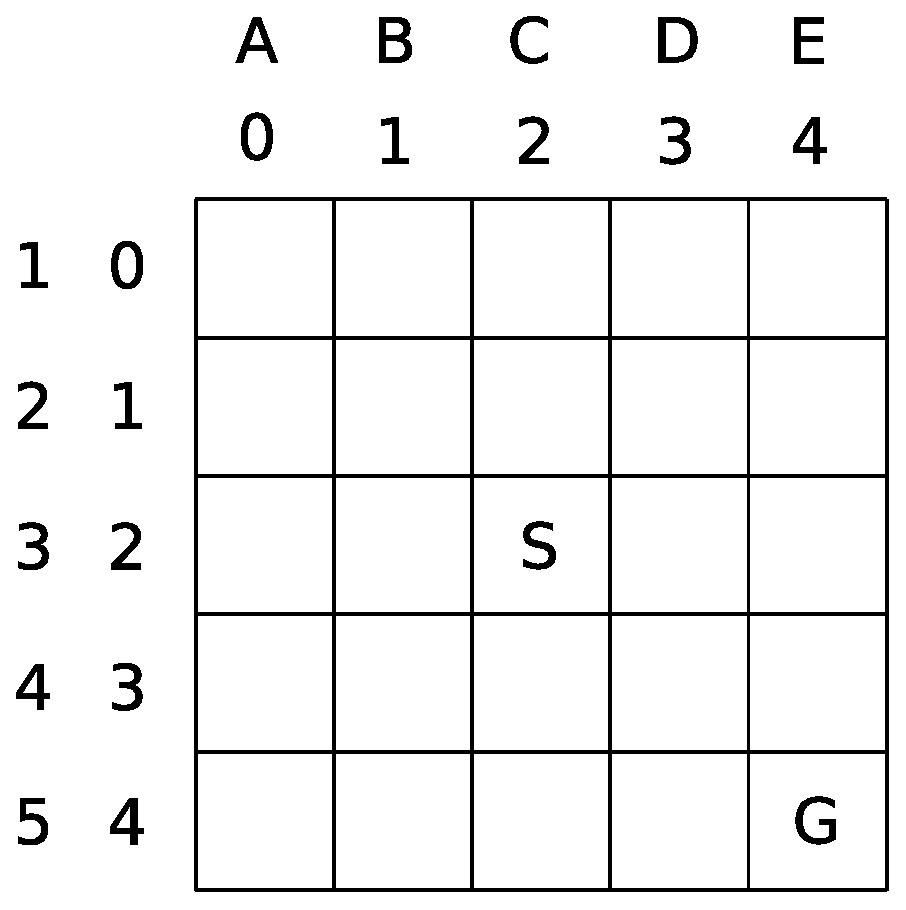
\includegraphics[width=0.25\textwidth]{./figures/drawing_v1.eps}
    \caption{Schematic of the problem.}
    \label{fig:problem}
\end{figure}

For future reference, if we linearly index the squares of the chessboard from 
$0$ to $24$ in a row-major fashion, then the mapping from the linear index to
the $(i, j)$ coordinates and back is given by the following bijections:

\begin{equation}
5j + i = k \leftrightarrow \left(i = k - 5 \floor*{\frac{k}{5}}, j = \floor*{\frac{k}{5}}\right) 
\label{eq:bijection}
\end{equation}
